\section{Binary System Data}
\label{sec:data}

\lorena{The training dataset represents $\sim 142,000$ binary systems comprised
of BBHs, BNSs, and NSBHs. The injections of these systems come from the Mock
Data Challenge (MDC) conducted during LIGO's second observing run (O2) and are
recovered using \texttt{GstLAL}, a low-latency detection pipeline. Regression is 
applied to four features, namely the initial masses $m_1$ and $m_2$ and the initial 
spin magnitudes $\chi_1$ and $\chi_2$. The training data has masses in the
ranges  $m_1 = [1.01, 119]$ and $m_2 =  [0.81, 81]$ and spin components 
$\chi_{1,2} =  [-0.99, 0.99]$, as shown in Fig.~\ref{parameter_space}.
For testing we use a dataset that contains $\sim 61,000$ systems from the O2 
MDC with injections recovered by \texttt{GstLAL}.} 
%The second is used as an
%additional test of model robustness as it contains $18,311$ systems from the O3 
%MDC which are recovered by the \texttt{PyCBC}, \texttt{GstLAL}, and 
%\texttt{MBTAOnline} pipelines. The number of triggers recovered by these 
%three detection pipelines are $8,742$, $7,221$, and $2,348$, respectively.}

\begin{figure}
% python3 paper_plots.py -v --NN --plots parspace --parspace_colorful
	\centering
	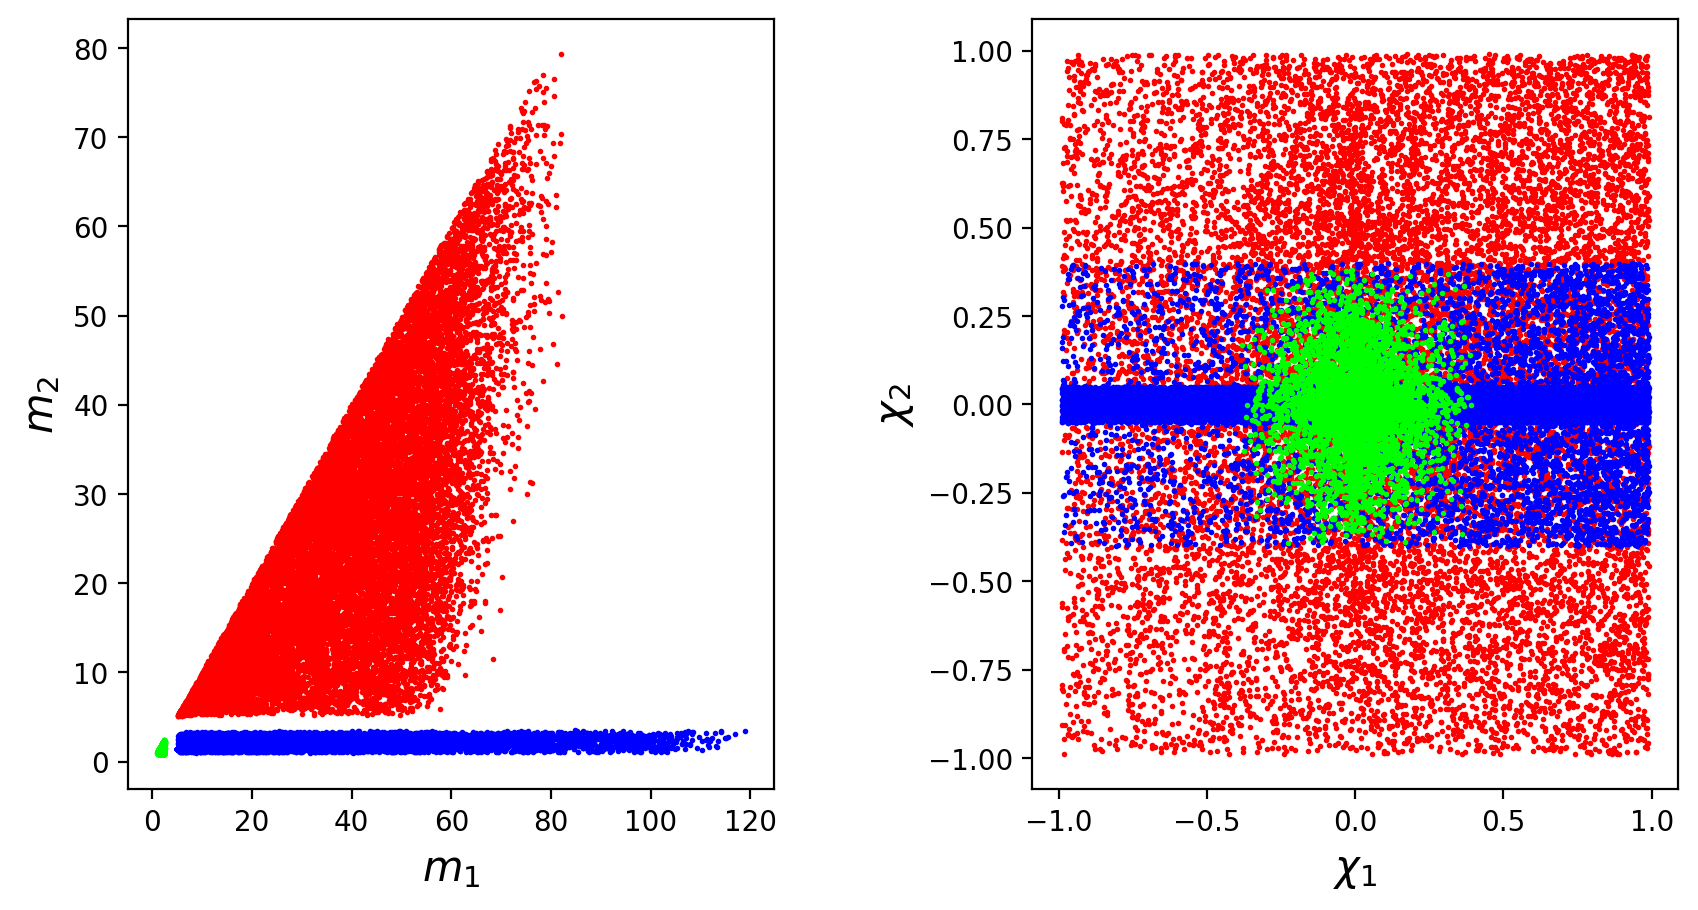
\includegraphics[width=0.45\textwidth]{training_parameter_space.png}
    \caption{The $m_1$-$m_2$ (left) and $\chi_1$-$\chi_2$ (right) parameter space 
		    of injections from the O2 MDC.
            }
	\label{parameter_space}
\end{figure}

\lorena{ML algorithms require the data to be standardized, i.e. have a zero
mean and unit variance. However, before standardizing the data we take an 
additional step to ensure astrophysical values from the predictions. In other 
words, a prediction without proper data conditioning can result in negative
masses and spin magnitudes greater than one. To avoid this, we first map the 
data to be in the $(0,1)$ range by solving a simple, linear system of equations 
separately for the masses and the spins. We, then, transform our data using a 
sigmoid function so that the values map between $(-\infty,+\infty)$. It
is only at this point that the data is ready to be standardized and fed into
the GPR and NN algorithms. Once the testing data predictions are completed, 
the reverse process is applied, i.e., the data is scaled back from 
standardization, exponentiated, and mapped back from $(0,1)$ to astrophysical 
values.}
